\chapter{Upgrade of the Upstream Tracker}
\label{ref:ut}

Located in the fringing fields in front of the LHCb dipole Magnet,
the Upstream Tracker (UT) plays an important role in improving the tracking
quality and speeding up trigger decisions:
Combining hits from VELO, SciFi, and UT provides the best \pt resolution
and reduce the rate of random combinations from VELO and SciFi to form
ghost tracks to about one fourth.
Furthermore, combining hits from VELO and UT removes low-\pt tracks and narrows
down the hit search window in SciFi, allowing for a faster track reconstruction
which leads to faster trigger decisions.

The University of Maryland group is responsible for the design, testing, and
commissioning of the readout and power regulating electronics;
An overview of the UT, discussed in \cref{ref:ut:overview},
will summarize the specifications and utilities of these electronics,
together with the sensors.
The author is tasked to test and develop quality assurance procedure for
the electronics that is responsible for
data acquisition and control of the UT detector.
In doing so, the author gained understanding on these functionalities of the UT.
The first functionality, data acquisition, is discussed in \cref{ref:ut:daq};
the second control functionality is described in \cref{ref:ut:ctrl}.


\section{Overview of the UT detector}
\label{ref:ut:overview}

The UT consists of 4 planar detection layers with full LHCb acceptance coverage.
As shown in \cref{fig:ut-layers},
the first and last layers are vertical,
whereas the second and third are rotated by a stereo angle of $\pm 5^\circ$
to form a $x$-$u$-$v$-$x$ configuration.

\begin{figure}[!htb]
    \centering
    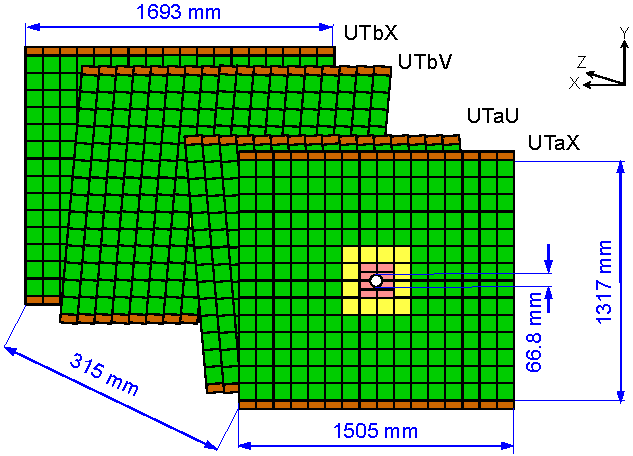
\includegraphics[width=0.7\textwidth]{./figs-lhcb-upgrade-overview/tracking/ut_upgrade.pdf}
    \caption{
        Four detection layers of UT,
        arranged in a $x$-$u$-$v$-$x$ configuration.
    }
    \label{fig:ut-layers}
\end{figure}

\subsection{Stave}


\subsection{PEPI}


\subsection{LVR}


\section{Data acquisition in UT}
\label{ref:ut:daq}

\subsection{More on DCB}


\subsection{TELL40 the event builder}


\subsection{Data transmission path}


\section{Control system of UT}
\label{ref:ut:ctrl}


\subsection{Timing and Fast Control (TFC)}


\subsection{Slow control for detector initialization and monitoring}
